\begin{figure}
\small
\centering
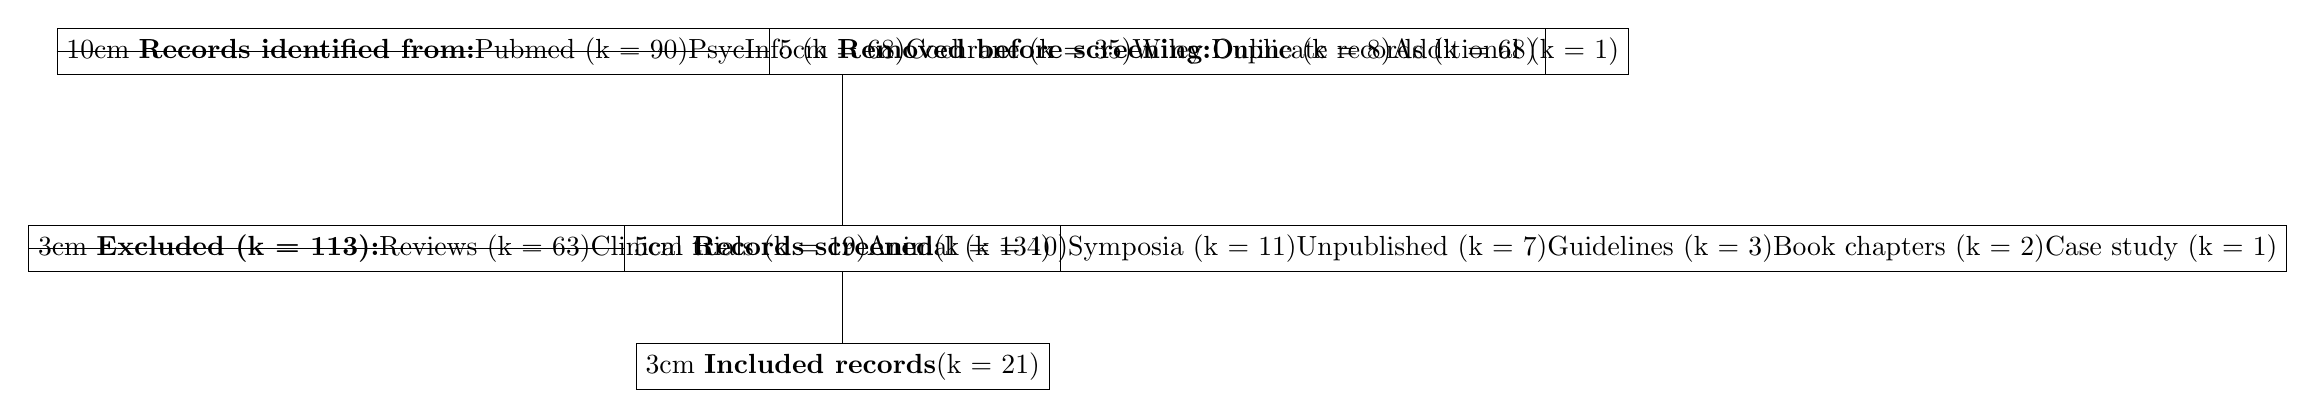
\begin{tikzpicture}[level distance = 40mm,sibling distance = 5mm]
%%%%%%%%%%%%%%%%%%%%%%%%%%%%%%%%%%%%%%%%%%%%
%%%%%%%%%%%%%%% BOXES %%%%%%%%%%%%%%%%%%%%%%%
% LEVEL 1 %%%%%%%%%%%%%%%%%%%%%%%%%%%%%%%%%%%%%%%%%%%ù
\node (1) at (-1,0)[draw]{\pbox{10cm}{
\textbf{Records identified from:}\\
Pubmed (k = 90)\\
PsycInfo (k = 68)\\
Cochrane (k = 35)\\
Wiley Online (k = 8)\\
Additional (k = 1)
}}
%_________________________________________________
child[grow = right]{node[draw]{\pbox{5cm}{
\textbf{Removed before screening:} \\
Duplicate records (k = 68)
}}} ;
% LEVEL 2 %%%%%%%%%%%%%%%%%%%%%%%%%%%%%%%%%%%%%%%%%%%%%%%%
\node (3) at (-1,-2.5) [draw]{\pbox{5cm}{
\textbf{Records screened}\\
(k = 134)
}}
%_______________________________________________
child[grow = right]{node[draw]{\pbox{3cm}{
\textbf{Excluded (k =  113):}\\
Reviews (k = 63)\\
Clinical trials (k = 19)\\
Animal (k = 10)\\
Symposia (k = 11)\\
Unpublished (k = 7)\\
Guidelines (k = 3)\\
Book chapters (k = 2)\\
Case study (k = 1)
}}} ;
% LEVEL 3 %%%%%%%%%%%%%%%%%%%%%%%%%%%%%%%%%%%%%%%%%%%%%%%%%%%%%%%%
\node (4) at (-1,-4) [draw]{\pbox{3cm}{
\textbf{Included records}\\ 
(k = 21) 
}} ;

%%%%%%%%%%%%%%%%%%%%%%%%%%%%%%%%%%%%%%%%%%%%
%%%%%%%%%% ARROWS %%%%%%%%%%%%%%%%%%%%%
%%%%%%%%%%%%%%%%%%%%%%%%%%%%%%%%%%%%%%%%%%%%
\draw (node cs:name = 1,anchor = south)
|- (-1,-1) -| (node cs:name = {3},anchor = north);

\draw (node cs:name = {3},anchor = south)
|- (-1,-3) -| (node cs:name = {4},anchor = north);

\end{tikzpicture}
\caption{Flow chart}
\label{fig:flowchart}
\end{figure}